\begin{figure}
    \centering
    \setlength{\resLen}{1.15in}
    \addtolength{\tabcolsep}{-6pt}
    \begin{tabular}{ccc}
        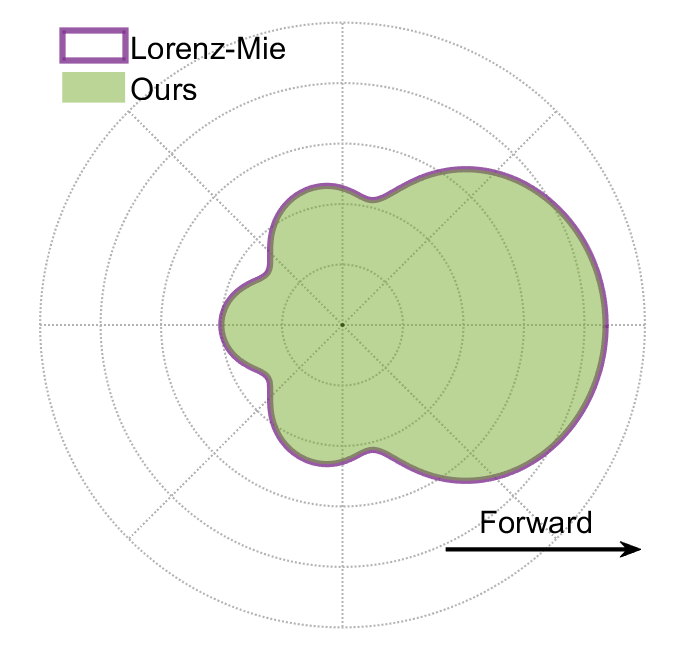
\includegraphics[width=\resLen]{pfunc/mie_300nm.png} & 
        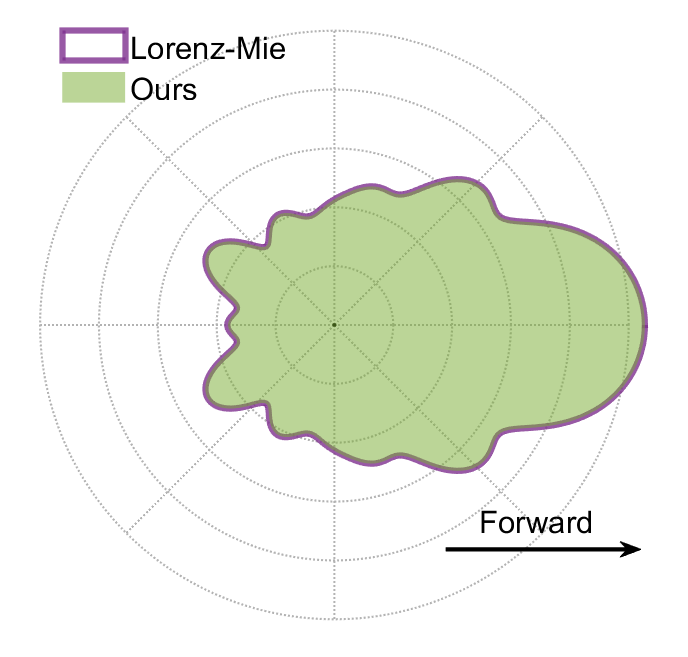
\includegraphics[width=\resLen]{pfunc/mie_600nm.png} &  
        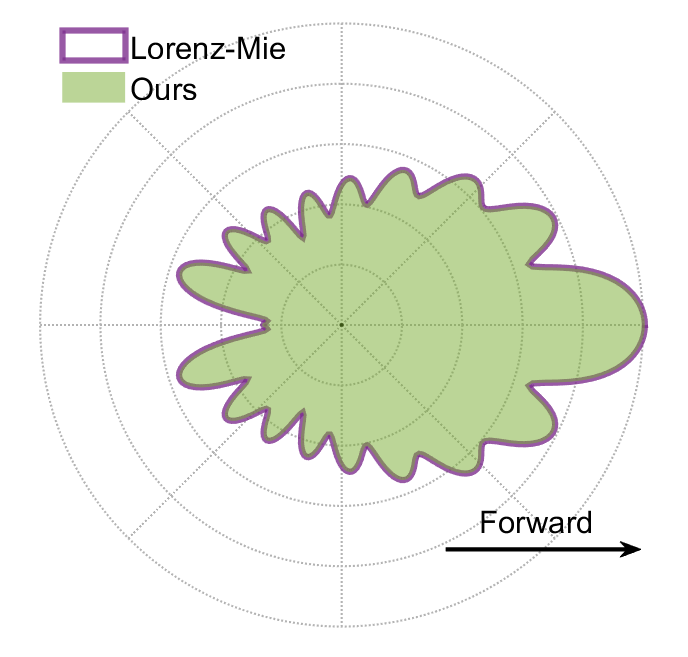
\includegraphics[width=\resLen]{pfunc/mie_900nm.png}  
        \\
        300nm & 600nm & 900nm
    \end{tabular}
    \caption{\label{fig:mie}
    Comparison against Lorenz-Mie theory: We compare our method with clusters containing a single particle (i.e., $\Ncls=1$) against a reference solution based on Lorenz-Mie theory for three different particle radii~$\radius_i \in \{ \text{300nm, 600nm, 900nm} \}$. As expected, for a single particle our method reduces to the same results as Lorenz-Mie theory. The wavelength is $\lambda=600$nm, while the refractive index of the particle is $\sIOR=1.5+0.1\img$.  
}
\end{figure}
